\section{Atividades}

Neste módulo, foram realizadas atividades práticas voltadas à automação de
tarefas, reutilização de código e exploração de ferramentas de desenvolvimento
e segurança em ambientes Kali Linux e Windows Server 2022. As tarefas
envolveram o reuso de código em Python para processamento de imagens,
instalação e exploração do JDK e da IDE NetBeans, automação de relatórios em
Linux, análise de assinaturas de malware com ClamAV e automação de tarefas
administrativas com PowerShell no Windows Server. O objetivo foi compreender,
na prática, como scripts e ferramentas de desenvolvimento podem ser utilizados
para otimizar processos, coletar informações do sistema e fortalecer a
administração de ambientes computacionais.

\newpage

\question[Atividade 6.1]{Exemplo de Reuso de Código em Python no Kali Linux}

\begin{figure}[H]
  \centering
  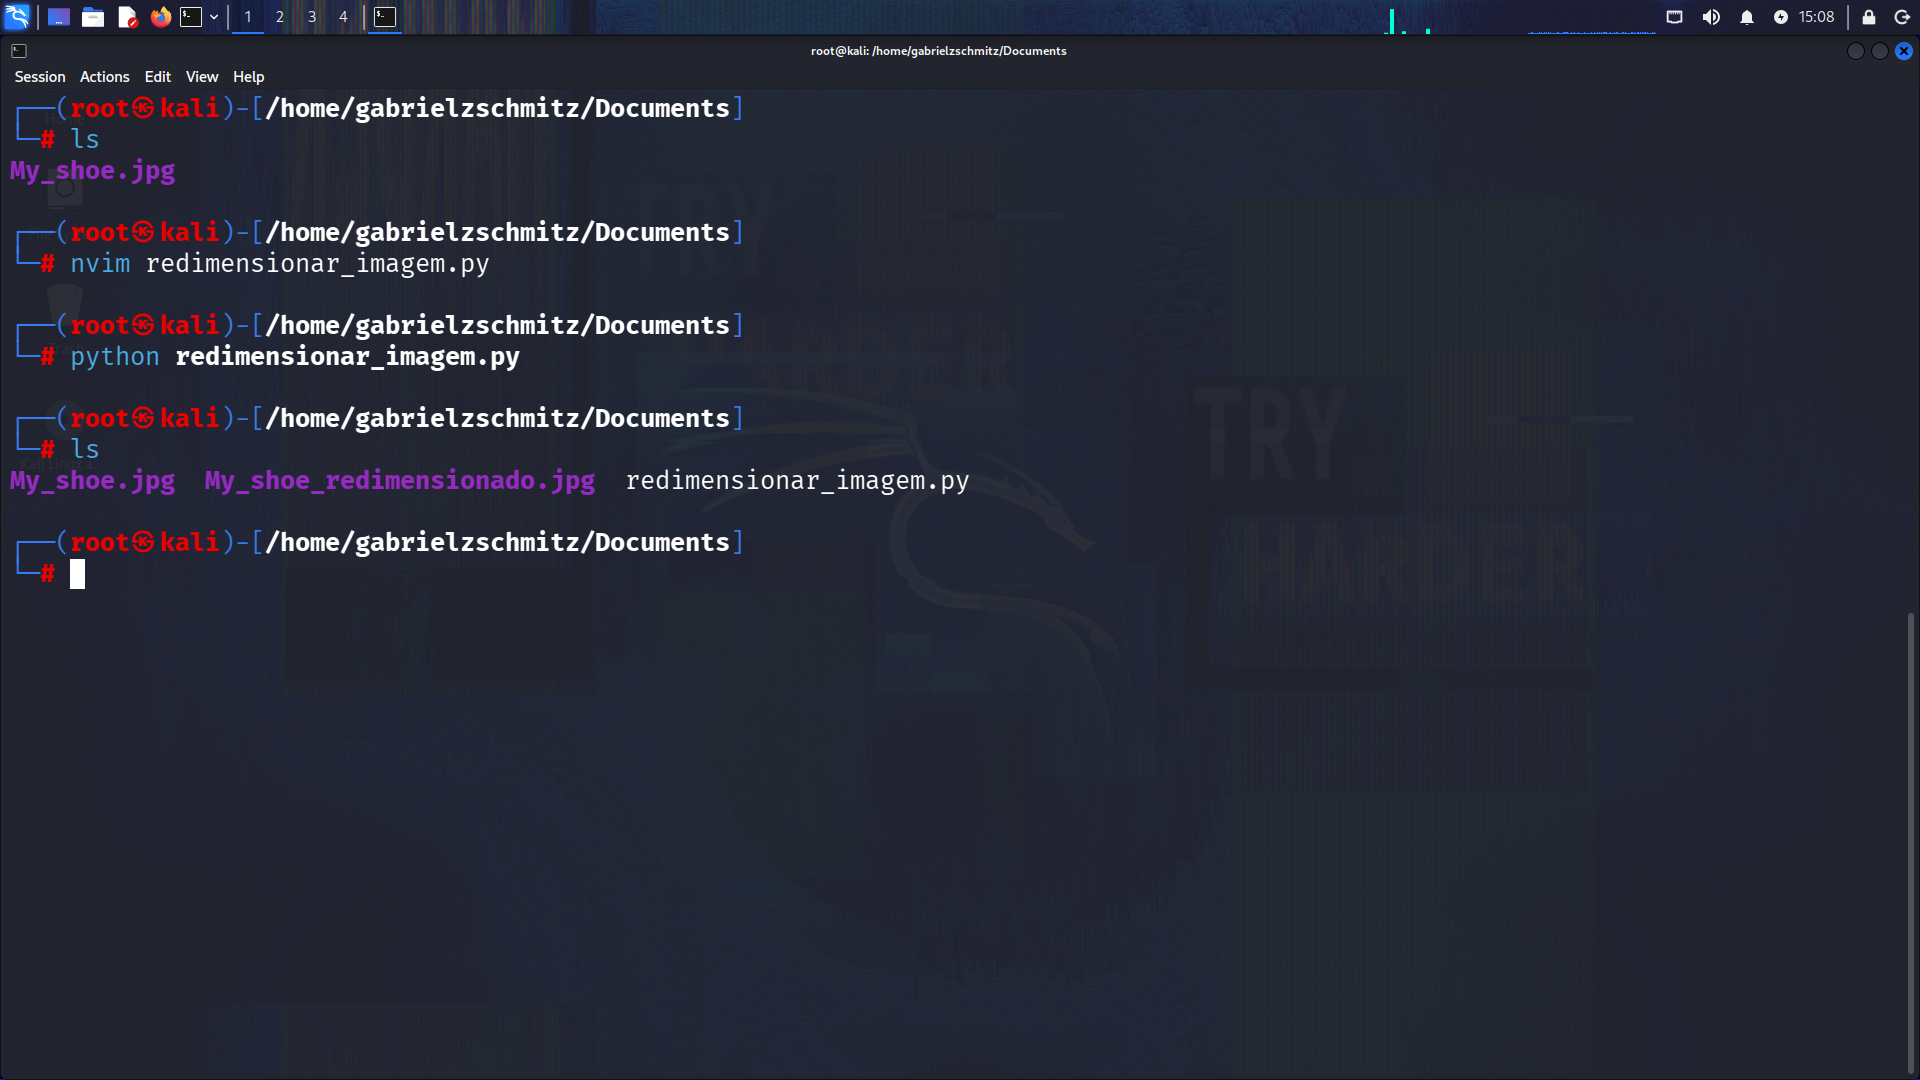
\includegraphics[width=0.99\textwidth]{./fig/fig6.1.png}
  \caption{Execução do script redimensionar_imagem.py e criação da imagem My\_shoe\_redimensionado.jpg}
  \label{fig:fig6.1}
\end{figure}


\newpage

\question[Atividade 6.2]{Conhecendo o SDK do Java (JDK) e um IDE no Kali Linux}

\begin{figure}[H]
  \centering
  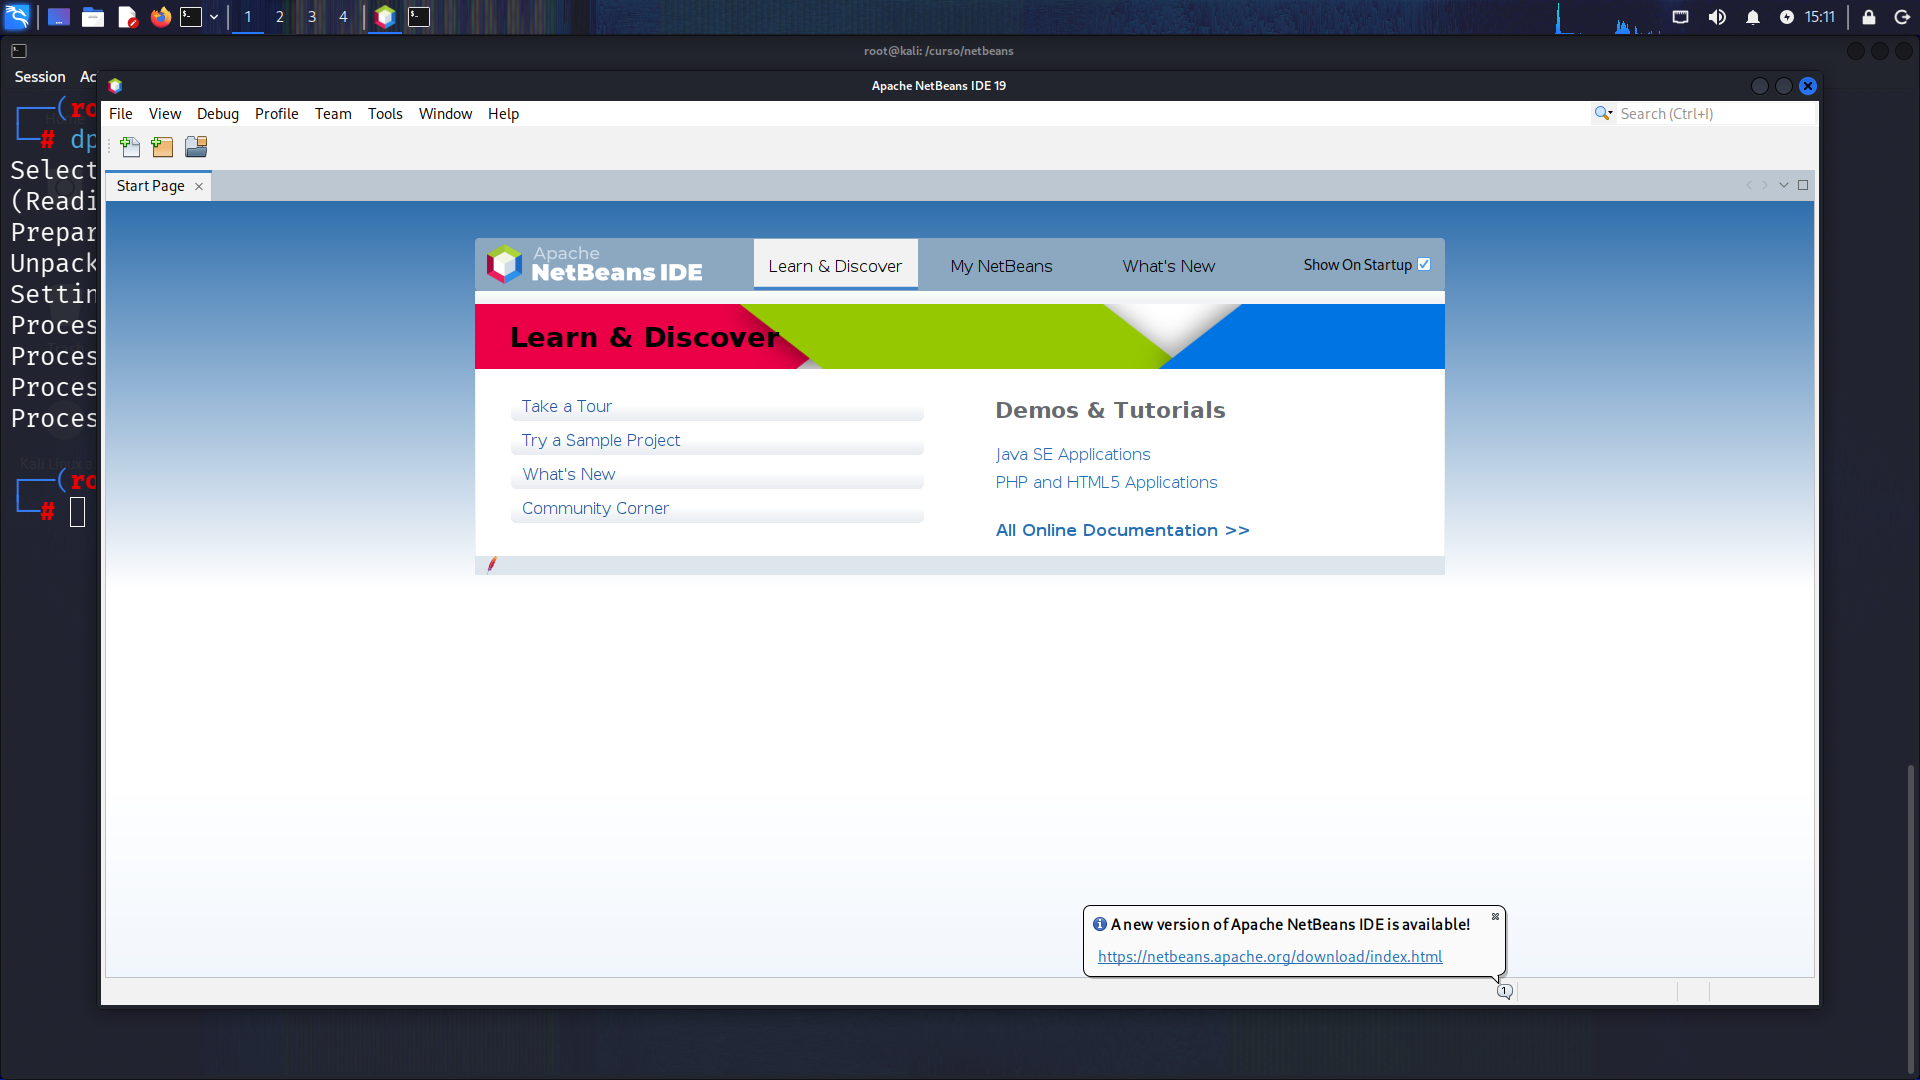
\includegraphics[width=0.99\textwidth]{./fig/fig6.2.png}
  \caption{Execução do Apache NetBeans IDE no Kali Linux}
  \label{fig:fig6.2}
\end{figure}


\newpage

\question[Atividade 6.3]{Automação de Tarefas com Python no Kali Linux}

\begin{figure}[H]
  \centering
  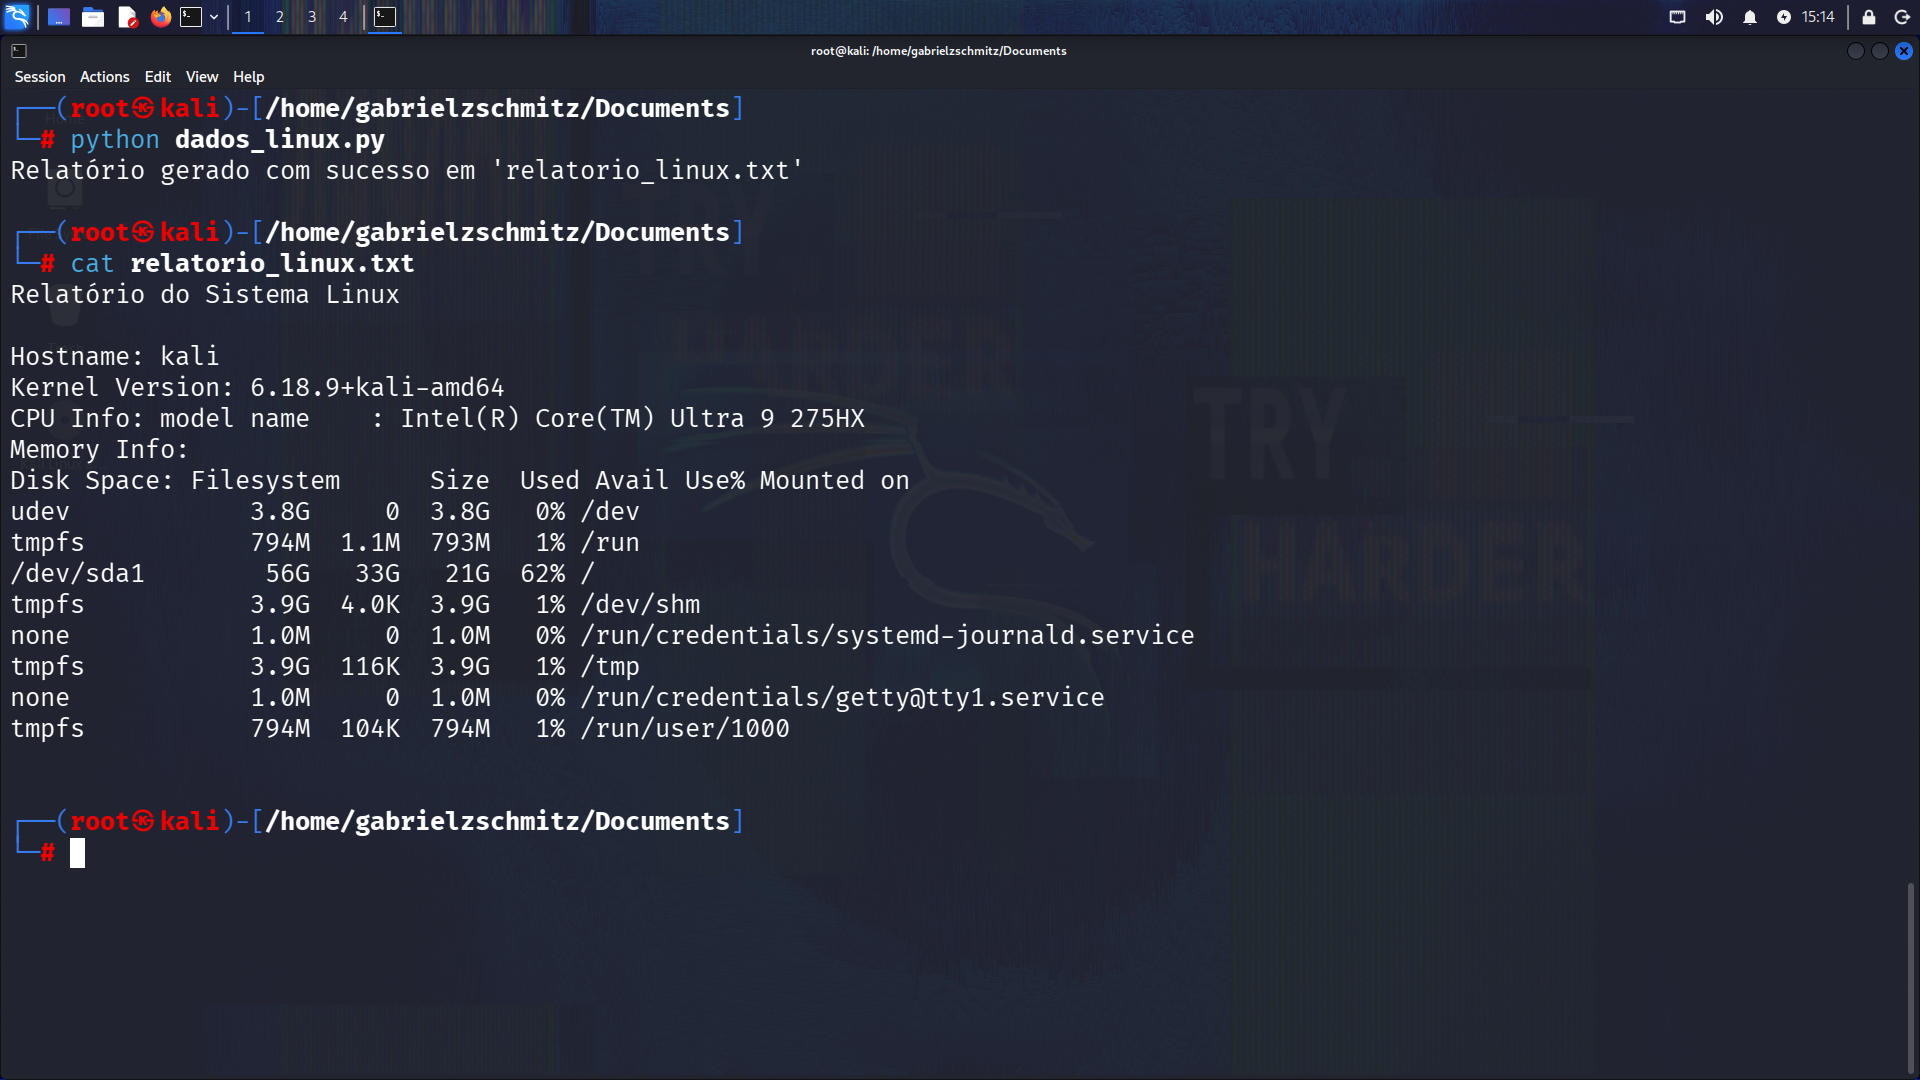
\includegraphics[width=0.99\textwidth]{./fig/fig6.3.png}
  \caption{Visualização do arquivo relatorio\_linux.txt contendo informações de hardware do sistema}
  \label{fig:fig6.3}
\end{figure}


\newpage

\question[Atividade 6.4]{Conhecendo o Antivírus ClamAV e sua Assinatura de Malware no Kali Linux}

\begin{figure}[H]
  \centering
  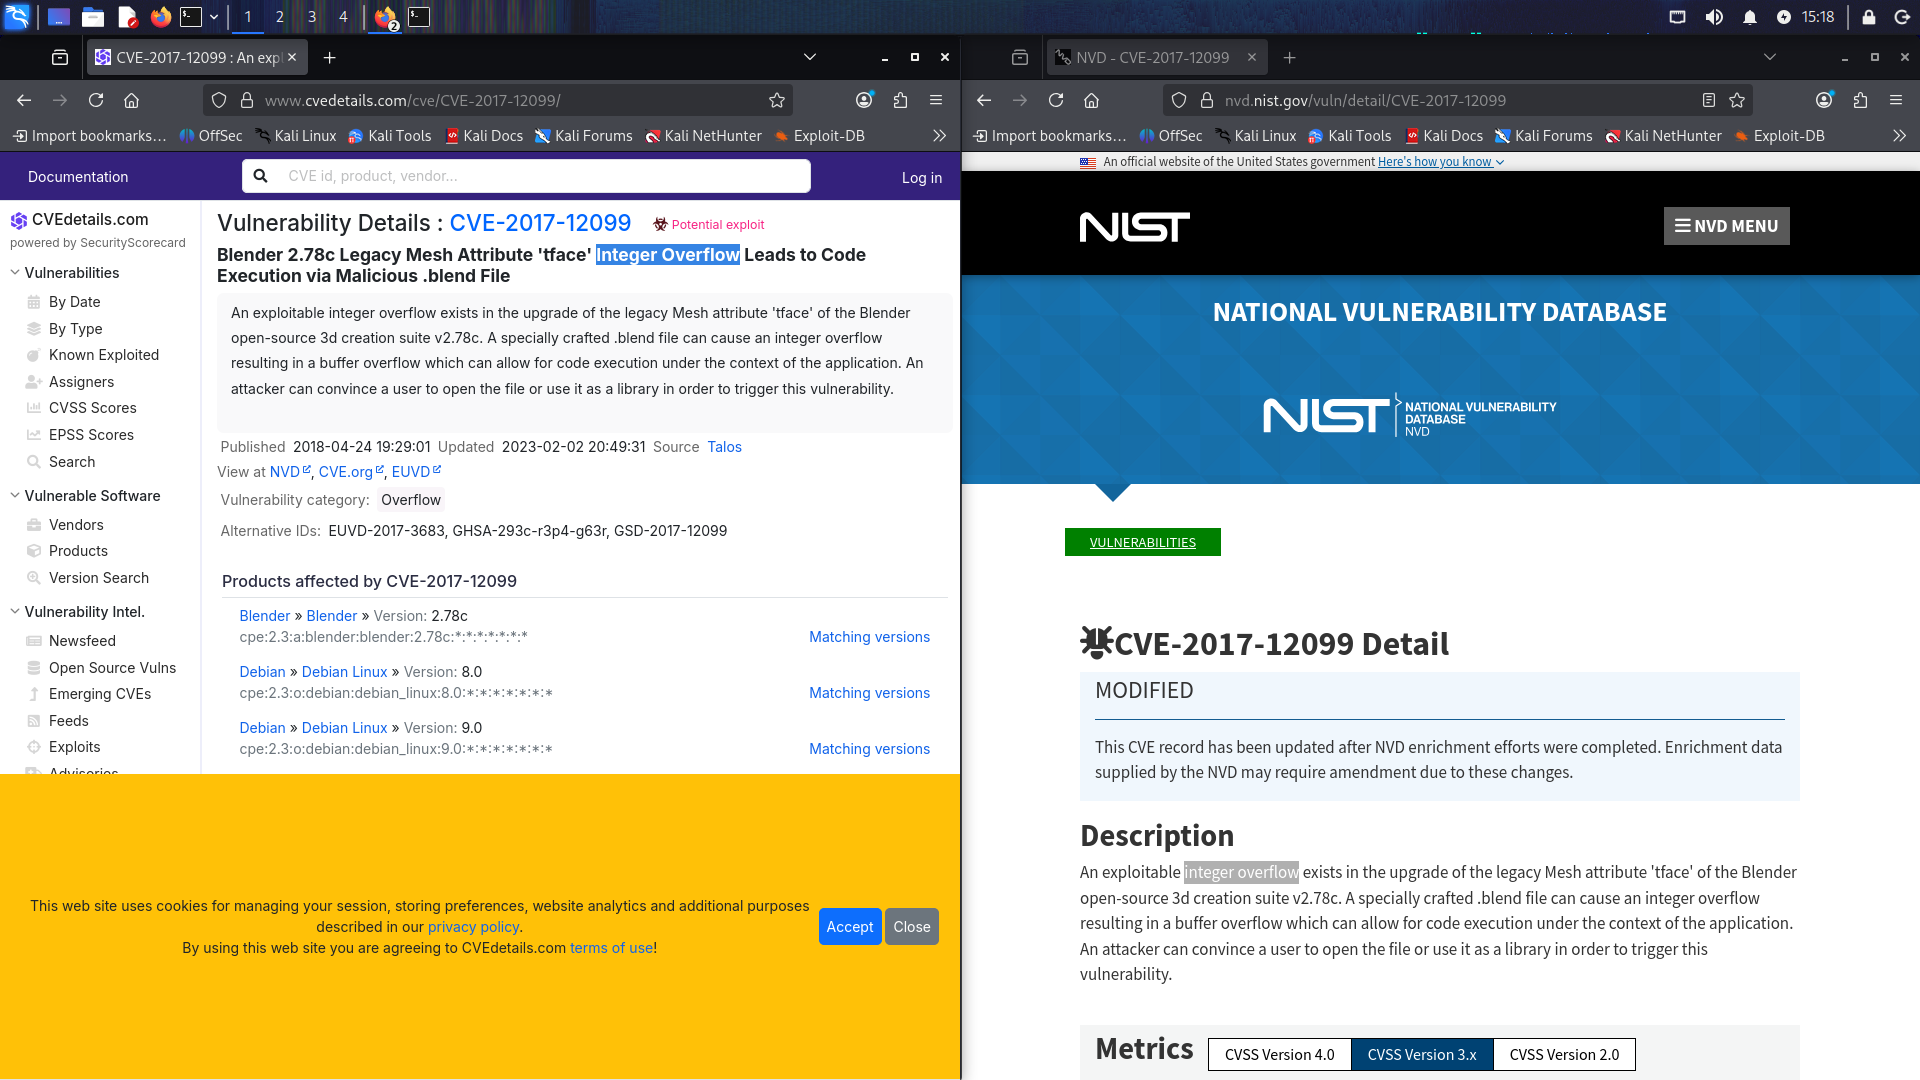
\includegraphics[width=0.99\textwidth]{./fig/fig6.4.png}
  \caption{Consulta da vulnerabilidade CVE-2017-12099 e identificação do tipo de ataque Integer Overflow}
  \label{fig:fig6.4}
\end{figure}


\newpage

\question[Atividade 6.5]{Automação de Tarefas com PowerShell no Windows Server 2022}

\begin{figure}[H]
  \centering
  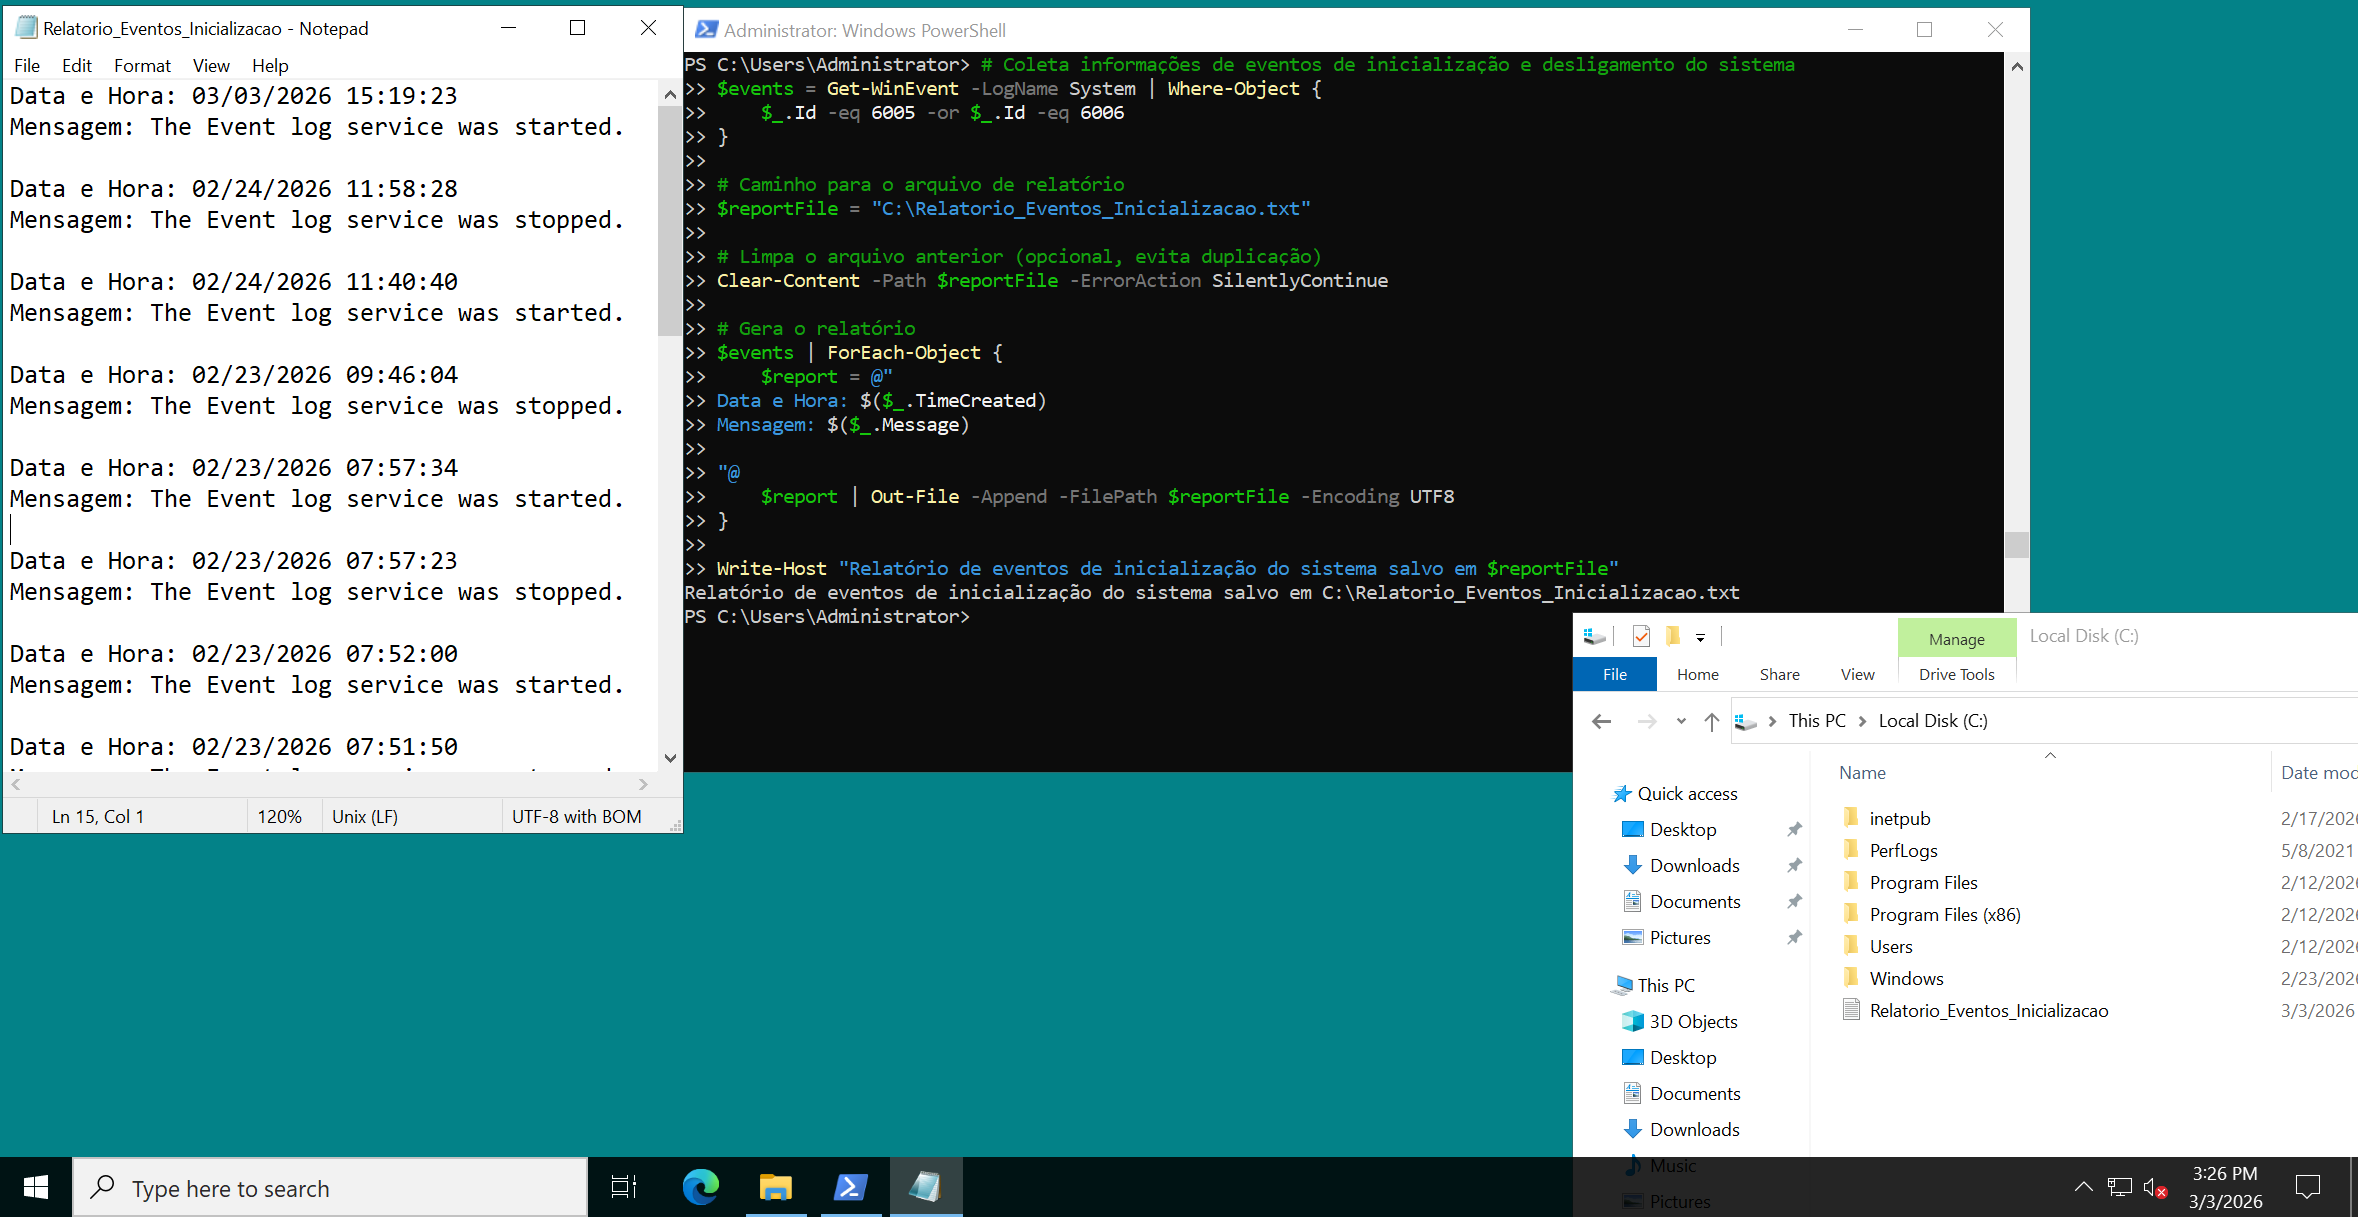
\includegraphics[width=0.99\textwidth]{./fig/fig6.5.png}
  \caption{Visualização do arquivo Relatorio\_Eventos\_Inicializacao.txt contendo logs de inicialização do sistema}
  \label{fig:fig6.5}
\end{figure}
